\part{Complex-Numbers-I}
\lecture{Complex Numbers I}{Complex-Numbers-I}
\section{Complex Numbers}

\title{Ordinary Differential Equations}
\subtitle{Math 232 - Week 4, Day 1}
\date{16 September 2013}

\begin{frame}
  \titlepage
\end{frame}

\begin{frame}
  \frametitle{Outline}
  \tableofcontents[currentsection]
\end{frame}


\subsection{The Letter i}


\begin{frame}
  \frametitle{The Letter i}

  Definition: 
  \begin{eqnarray*}
    i & = & \sqrt{-1} 
  \end{eqnarray*}

  Which means....
  \begin{eqnarray*}
    i^2 & = & -1
  \end{eqnarray*}

\end{frame}


\begin{frame}
  \frametitle{Complex Numbers}

  \begin{definition}
    A \redText{complex number} is a number that can be expressed as
    \begin{eqnarray*}
      a + bi,
    \end{eqnarray*}
    where $a$ and $b$ are real numbers.
  \end{definition}


\end{frame}



\begin{frame}
  \frametitle{Example}

  \begin{eqnarray*}
    z_1 & = & 3 + 2i \\
    z_2 & = & 5 - 7i
  \end{eqnarray*}

\end{frame}

\subsection{Operations With Complex Numbers}

\begin{frame}
  \frametitle{Addition}

  \begin{eqnarray*}
    (3+2i) + (5-7i) & = & 
    \uncover<2->{%
      (3+5) + (2-7)i \\
      & = & 8 - 5i\\
    }
    ~ \\
    (4-2i) + (6-3i) & = & 
    \uncover<3->{%
      (4+6) + (-2-3)i \\
      & = & 10 - 5i
    } 
  \end{eqnarray*}

\end{frame}

\begin{frame}
  \frametitle{Multiplication}

  \begin{eqnarray*}
    (3+2i)(5-7i) & = & 
    \uncover<2->{%
      15 + 10i - 21i - 14 i^2 \\
      & = & 15 - 11i + 14 \\
      & = & 29 - 11 i
    }
  \end{eqnarray*}

  \begin{eqnarray*}
    (4-2i)(6+3i) & = & 
    \uncover<3->{%
      24 - 12i + 12 i - 6i^2 \\
      & = & 24 + 6 \\
      & = & 30
    }
  \end{eqnarray*}

\end{frame}


\subsection{Complex Conjugate}

\begin{frame}
  \frametitle{The Complex Conjugate}

  \begin{definition}
    The \redText{complex conjugate} of $z$, denoted $\bar{z}$, is
    found by reversing the sign of the imaginary part.
  \end{definition}

  
  Example:
  For each of the numbers given below:
  \begin{eqnarray*}
    z_1 & = & 3 + 2i, \\
    z_2 & = & 5 - 6i, 
  \end{eqnarray*}
  the complex conjugates are the following:
  \begin{eqnarray*}
    \bar{z_1} & = & 3 - 2i, \\
    \bar{z_2} & = & 5 + 6i.
  \end{eqnarray*}


\end{frame}

\begin{frame}
  \frametitle{Special Property of the Complex Conjugate}

  \begin{eqnarray*}
    z\cdot\bar{z} & = & (a+bi)(a-bi) \\
    & = & a^2 +abi - abi - b^2 i^2 \\
    & = & a^2 + b^2
  \end{eqnarray*}

\end{frame}



\begin{frame}
  \frametitle{So What?}

  \begin{eqnarray*}
    \frac{5-3i}{2+3i} & = & 
    \uncover<2->{%
      \frac{(5-3i)(2-3i)}{(2+3i)(2-3i)} \\
      & = & \frac{10-6i-15i+9i^2}{4+6i-6i-9i^2} \\
      & = & \frac{1-21i}{13} \\
      & = & \frac{1}{13} - \frac{21}{13} i
    }
  \end{eqnarray*}

\end{frame}

\begin{frame}
  \frametitle{Example}

  \begin{eqnarray*}
    \frac{2+3i}{5-3i} & = & 
    \uncover<2->{%
      \frac{(2+3i)(5+3i)}{(5-3i)(5+3i)} \\
      & = & \frac{10+15i+6i+9i^2}{25-15i+15i-9i^2} \\
      & = & \frac{1+21i}{34} \\
      & = & \frac{1}{34} + \frac{21}{34}i
    }
  \end{eqnarray*}

\end{frame}

\subsection{Graphical View of Complex Numbers}

\begin{frame}
  \frametitle{Graphical View of Complex Numbers}

  \only<1>{\centerline{\includegraphics[width=4cm]{img/complexPlane}}}
  \only<2>{\centerline{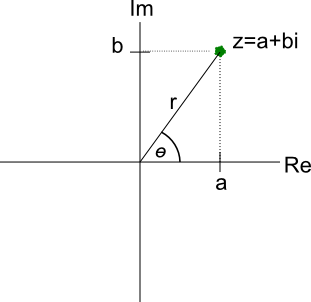
\includegraphics[width=4cm]{img/complexPlanePolar}}}
  
  \begin{eqnarray*}
    a & = & r\cos(\theta) \\
    b & = & r\sin(\theta) \\
    r & = & \sqrt{a^2+b^2} \\
    \tan(\theta) & = & \frac{b}{a}
  \end{eqnarray*}
  (Be careful about the arctangent. Your calculator lies!)

\end{frame}


\begin{frame}
  \frametitle{Example}

  \begin{eqnarray*}
    z & = &  2 + 2i
  \end{eqnarray*}

  \uncover<2->
  {%

    \begin{eqnarray*}
      r & = & \sqrt{2^2+2^2}, \\
        & = & 2\sqrt{2}, \\
      \tan(\theta) & = & \frac{2}{2}, \\
      \theta       & = & \frac{\pi}{4}.
    \end{eqnarray*}

  }

\end{frame}


\iftoggle{clicker}{%
\begin{frame}
  \frametitle{Clicker Quiz}
    
      \ifnum\value{clickerQuiz}=1{%

        Determine the radius and angle for the following complex number:
          \begin{eqnarray*}
            z & = & -2 + 2i
          \end{eqnarray*}


          \begin{tabular}{l@{\hspace{3em}}l@{\hspace{1em}}l}
            A: &  $r=2$, & $\theta= -\pi/4$ \\
            B: &  $r=2$, & $\theta= 3\pi/4$ \\
            C: &  $r=2\sqrt{2}$, & $\theta= -\pi/4$ \\
            D: &  $r=2\sqrt{2}$, & $\theta= 3\pi/4$ \\ 
          \end{tabular}

     }\fi

     \ifnum\value{clickerQuiz}=2{%

        Determine the radius and angle for the following complex number:
          \begin{eqnarray*}
            z & = & -2 -2i
          \end{eqnarray*}


          \begin{tabular}{l@{\hspace{3em}}l@{\hspace{1em}}l}
            A: &  $r=2$, & $\theta= -\pi/4$ \\
            B: &  $r=2$, & $\theta= 5\pi/4$ \\
            C: &  $r=2\sqrt{2}$, & $\theta= -\pi/4$ \\
            D: &  $r=2\sqrt{2}$, & $\theta= 5\pi/4$ \\ 
          \end{tabular}

     }\fi

      \ifnum\value{clickerQuiz}=3{%

        Determine the radius and angle for the following complex number:
          \begin{eqnarray*}
            z & = & -2 + 2i
          \end{eqnarray*}


          \begin{tabular}{l@{\hspace{3em}}l@{\hspace{1em}}l}
            A: &  $r=2$, & $\theta= -\pi/4$ \\
            B: &  $r=2$, & $\theta= 3\pi/4$ \\
            C: &  $r=2\sqrt{2}$, & $\theta= -\pi/4$ \\
            D: &  $r=2\sqrt{2}$, & $\theta= 3\pi/4$ \\ 
          \end{tabular}


     }\fi

    \vfill
    \vfill
    \vfill

\end{frame}

}

    

\subsection{Euler's Formula}

\begin{frame}
  \frametitle{A Differential Equation}

  \textbf{Note: \redText{$i$ is a constant.}}
  \begin{eqnarray*}
    \Rightarrow \frac{d}{dt} e^{it} & = & i e^{it}.
  \end{eqnarray*}

  The function
  \begin{eqnarray*}
    y(t) & = & e^{it}
  \end{eqnarray*}
  is \textbf{\redText{the}} solution to the differential equation
  \begin{eqnarray*}
    y' & = & iy, \\
    y(0) & = & 1.
  \end{eqnarray*}

\end{frame}

\begin{frame}
  \frametitle{Another Solution}

  There is another solution,
  \begin{eqnarray*}
    y(t) & = & \cos(t) + i \sin(t).
  \end{eqnarray*}

  \begin{eqnarray*}
    \frac{d}{dt} y(t) & = & -\sin(t) + i \cos(t), \\
    y(0) & = & \cos(0) + i\sin(0) \\
    & = & 1.
  \end{eqnarray*}

\end{frame}


\begin{frame}
  \frametitle{Euler's Formula}

  \begin{block}{Euler's Formula}
    \begin{eqnarray*}
      e^{it} & = & \cos(t) + i\sin(t)
    \end{eqnarray*}
  \end{block}

  \vfill

  An alternative way to express Euler's Formula:
  \begin{eqnarray*}
    e^{i\theta} & = & \cos(\theta) + i\sin(\theta).
  \end{eqnarray*}
  
\end{frame}

\begin{frame}
  \frametitle{Another way to express complex numbers}

  Suppose we have
  \begin{eqnarray*}
    z & = & a + bi, \\
    & = & r\cos(\theta) + ir\sin(\theta) \\
    & = & r \lp \cos(\theta) + i\sin(\theta) \rp \\
    & = & r e^{i\theta}
  \end{eqnarray*}


  \begin{definition}
    The \redText{Euler Form} for a complex number is
    \begin{eqnarray*}
      z & = & r e^{i\theta},
    \end{eqnarray*}
    where $r$ is the radius and $\theta$ is the angle from the polar
    form of the number.
  \end{definition}

\end{frame}

\begin{frame}
  \frametitle{Example}
  
  \begin{eqnarray*}
    z & = & 2 + 2i \\
    \uncover<2->
    {%
       & = & 2\sqrt{2} \cos(\pi/4) + i 2\sqrt{2} \sin(\pi/4) \\
       & = & 2\sqrt{2} \lp \cos(\pi/4) + i\sin(pi/4) \rp \\
       & = & 2\sqrt{2} e^{i\pi/4}
    }
  \end{eqnarray*}

  % TODO - add a picture of the point in the complex plane
\end{frame}

\begin{frame}
  \frametitle{Example}
  \begin{eqnarray*}
    z & = & \sqrt{3} + i  \\
    \uncover<2->
    {%
         & = & 2 \cos\lp\frac{\pi}{6}\rp + i 2 \sin\lp\frac{\pi}{6}\rp, \\
         & = & 2 e^{i\frac{\pi}{6}}.
    }
  \end{eqnarray*}
  % TODO - add a picture of the point in the complex plane
\end{frame}

\iftoggle{clicker}{%
\begin{frame}
  \frametitle{Clicker Quiz}
    
      \ifnum\value{clickerQuiz}=1{%

        Express -1 in Euler form.

          \begin{tabular}{l@{\hspace{3em}}l}
            A: &  $e^{-i\pi}$, \\
            B: &  $e^{-i\pi/2}$, \\
            C: &  $e^{-i}$, \\
            D: &  $-1$, \\ 
          \end{tabular}

     }\fi

     \ifnum\value{clickerQuiz}=2{%

        Express -1 in Euler form.

          \begin{tabular}{l@{\hspace{3em}}l}
            A: &  $e^{-i\pi}$, \\
            B: &  $e^{-i\pi/2}$, \\
            C: &  $e^{-i}$, \\
            D: &  $-1$, \\ 
          \end{tabular}


     }\fi

      \ifnum\value{clickerQuiz}=3{%

        Express -1 in Euler form.

          \begin{tabular}{l@{\hspace{3em}}l}
            A: &  $e^{-i\pi}$, \\
            B: &  $e^{-i\pi/2}$, \\
            C: &  $e^{-i}$, \\
            D: &  $-1$, \\ 
          \end{tabular}


     }\fi

    \vfill
    \vfill
    \vfill

\end{frame}

}


\begin{frame}{Ominous Foreshadowing}

  What \textbf{\redText{are}} the cube root\textbf{\redText{s}} of
  one?

  \uncover<2->{
    \begin{eqnarray*}
      1,~e^{i2\pi/3},~e^{i4\pi/3}.
    \end{eqnarray*}
  }

  \uncover<3->{
    Because...
    \begin{eqnarray*}
      1^3 & = & 1, \\
      \lp e^{i2\pi/3}\rp^3 & = & e^{i2\pi}~=~1, \\
      \lp e^{i4\pi/3}\rp^3 & = & e^{i4\pi}~=~1.
    \end{eqnarray*}
  }

  \uncover<4->{ruh roh...}
  
\end{frame}


% LocalWords:  Clarkson pausesection hideothersubsections
